 
This work on using Gaussian Process for cosmic shear analysis 
was first discussed as a possibility in  \citep{Schneider2014}  and 
forms the basis of the analyses that I helped perform 
in Schneider et al. (in prep.). 

\section{Introduction} 

% why study cosmic shear 
A cornerstone of cosmology is found on the 
observation of the highly Gaussian temperature fluctuations in the cosmic microwave 
background (CMB), an ancient light emitted during the recombination in the early
universe. Many physical models can explain how these
nearly Gaussian fluctuations could arise from quantum perturbations in the 
early universe. Furthermore, we know how these perturbations could grow
through linear transfer over time to form a large-scale ($> 10 h^{-1} Mpc$) 
dark matter (DM) density field that is consistent with present
day observables. 
This cosmic web encodes valuable information for constraining cosmological
parameters. such as the matter density ($\Omega_m$) and the fluctuation amplitude 
of the matter density ($\sigma_8$) on a particular characteristic scale (8
$h^{-1} Mpc$). 
% The observable, the subtle distortion signals of galaxy shapes 
% that is induced by the gravity of intervening DM
% between far away galaxies and the observers, is also known as cosmic shear.  

% as the Large Synoptic Survey Telescope (LSST) will
% provide data of high enough quality and large enough volume such that the
% constraints will be systematics limited. 
% how complicated is cosmic shear inference 
% Past analyses of large scale structures, such as
% the Canadian-French-Haiwaiian Telescope Lens (CFHTLens;
% \citealt{Kilbinger2013}), the Deep Lens Survey
% (DLS; \citealt{Jee2013a}), the Dark Energy Survey (DES; \citealt{Abbott2016}) and others, 
% have already demonstrated the constraining power  
% constraints.
% This has sparked interests to
% come up with a comprehensive (statistical) framework to address the effects
% from systematics.

% As first discussed in chapter 1, the presence of DM could distort background
% galaxy shapes through gravitational lensing.
The analysis of the DM density field, however, is far from trivial. 
The galaxies those shapes distortions reflect the density of intervening DM, 
only provide a weak, indirect gravitational lensing signal (known as cosmic
shear; $\lensparams$). The signal is also buried among various sources of noise
and systematics. 
To improve the existing constraints, there are many ongoing 
efforts to refine the analysis pipeline. 
In this work, we propose a new, probabilistic approach for representing 
the cosmic shear information, 
and show how it can be used in a probabilistic framework. 
This can allow the joint inference of the signal, the noise and the systematics, 
and potentially provide a less biased estimate of the cosmological parameters 
(${\bf \theta}$). 
The most relevant reference of such a probabilistic approach can be found in 
\cite{Schneider2014} and Schneider et al. (in prep.), 
while an alternative hierarchical approach can be found in \cite{Alsing2015}. 

In general, an analysis framework for cosmic shear includes: \\ 
(1) the identification and deblending of source galaxies from sky survey data 
using software such as {\sc SEXtractor} \citep{Bertin1996}, {\sc Celeste}
\citep{Regier2014}, and / or {\sc Tractor} \citep{Lang2010}, among others;\\
(2) the measurement of the ellipticities of the tracer galaxies  
and the estimation of the measurement error ($\sigma_{\rm
ms}$) via some shape fitting routines; \\
(3) the characterization and correction of atmospheric aberrations and survey masking 
on the shapes of foreground stars using
 a point-spread-function (PSF, which is represented by $\Pi$ in this work; \citealt{Jee2013a}, \citealt{Rowe2010}); \\
(4) the representation of the intrinsic ellipticities of the tracer galaxies by a
distribution, which is usually assumed to be a Gaussian with zero mean
and a variance of $\sigma_e^2 \approx 0.25^2$;\\ 
(5) the estimation of the (photometric) redshift of the source galaxies. The 
estimates of the (photometric) redshift can be used to weight the lensing kernel
to reflect the different lensing efficiency when the DM overdensities 
are located at different distances from the observer and the source galaxies.
\\
% An alternative use of the redshift is for a tomographic analysis is performed
% to infer the three-dimensional DM density along the line-of-sight;\\
(6) the statistical inference and representation of the cosmic shear signal,
which is the main theme of this chapter;
and finally \\ 
(7) the (cosmological) simulation efforts for relating all the above contributions to isolate the cosmic shear signal and
estimate the underlying (Gaussian part) of the DM distribution. 
The non-Gaussian part of the DM distribution introduced by processes
such as gravitational collapse is also inferred from the simulations before    
cosmological constraints are obtained from a fit to a certain representation of
the cosmic shear information. 
% Even though we lay out the different stages of a cosmic shear analysis sequentially,
% performing the analysis separately may introduce unintended biases. This is
% because an estimation or a correction at separate stages may only provide a local
% best fit solution.   

% Even though the representation of the cosmic shear information on constituents
% one step in the entire pipeline, there are a large number of studies that try
% to improve the current methods. Most of the studies make use of summary 
% statistics. 

There are many proposals for how to best represent the cosmic shear information
(step 6). The technical details of each method differ, but most of them involve
making use of an estimator that provides a summary of the data.
Examples of commonly used estimators include, the two-point correlation function 
(2PCF) and the power spectrum, which is part of the Fourier transform of the 2PCF, 
the ring statistics, the aperture mass dispersion and the peak statistics.  
A detail discussion of each of them can be found in 
\cite{Kilbinger2013}, \cite{Bartelmann2001a}.
An important concern for computing the summary statistics of the cosmic shear 
comes from the lensing physics. As the lensing observables are the second derivatives of the
scalar potential under the Born approximation, we expect them to be curl-free
(i.e. only contain an E-mode, those name is analogous to the curl-free electric
field). An desired property of the representation of the
cosmic shear, is therefore to show a complete separation of the E-mode and the B-mode.
However, there can be various sources of the B-mode signals. A well known
cause of mode mixing is known as the finite-interval problem. It is due to
imperfect observation conditions, such as blending of galaxies at small scales,
or limitations from survey boundaries at large scales \citep{Kilbinger2013}.  
Specific computational implementation of the summary statistics (e.g. the ring
statistics or the 2PCF) that bins the 
observed shear can also mix the E and B-modes (\citealt{Eifler2010},
\citealt{Becker2013}). We provide a new model of cosmic shear that may
alleviate some of the aforementioned problems. 
 
With the use of two graphical models, we will demonstrate how our method
(step 6) may enable better joint inference with the other relevant parts (e.g. 2, 3, 4). 
The rest of this chapter will have the following structure, we will \\ 
1) illustrate the basic properties of the Gaussian Process, the model that we
use to represent the cosmic shear signal\\ 
2) show the derivation for incorporating the lensing physics in 
a suitable covariance kernel for a Gaussian Process;  
And in the process of describing our method, we will comment on how our method is  
similar or different from other approaches for cosmic shear inference. \\
3) lay out a hierarchical model for making several mass maps 
with the modified Gaussian Process and show some preliminary results \\ 
4) discuss the limitations and possible extensions to our method.\\
In no part of this work do we explicitly assume a cosmological model. All our
derivations follow from either the lensing physics or our statistical method.   
% Our method provides an alternative from having to use the 2PCF to represent the
% Gaussian portion of the cosmic shear information. 
% Source galaxies provide sparse constraints to probe the matter density along
% the line of sight. 

% how does the signal look like? E-mode ? E-mode?
% Uncorrected systematics can show up in the signal  
%  there is also discussion of the current approaches for
% representing the cosmic shear signal.
% There are current approach for representing  
% As we have demonstrated 
% Although our proposed method is only one of the many stages needed for accurate 
% cosmic shear inference, we try to put our method into context by providing two
% basic analyses. The examples will show how our method are related to other
% stages of the analyses (e.g. 2, 3, 4 and 7). 

\section{Method}

The crucial ingredient for describing cosmic shear is the deterministic
lensing physics. However, 
the choice of the representation of cosmic shear affects both the
inference procedure and the estimation of cosmological parameters. 


binning can cause the mixing of curl-free and the non-curl-free mode 
of the signal.
% The identification of the curl-free (E-mode) part of the signal that contain
% the gravitational lensing signal and the remaining B-mode 
% that can be caused by systematics or other  

\subsection{The basics of a Gaussian Process}
A Gaussian Process is one of the most studied and published 
generative model for non-parametric regression. 
It allows the inference of the joint probability density 
function (PDF) for describing a set of data. 
This gives the model the flexibility for a wide range
of successful applications in many fields. 
In Astronomy, a GP has been used for modeling 
the light curve of exoplanets from discrete data points \citep{Ambikasaran2014a}.
Or the GP can be used as a prior probability for optimizing the model parameters of
neural networks \citep{Snoek2012}. 
It has also been used for other classification, dimensionality reduction 
and pattern extraction tasks
with state-of-the-art predictive performance 
(\citealt{Wilson2013}, \citealt{Duvenaud2013}, \citealt{Rasmussen2006}).
We focus our analyses on how the GP can be utilized to compute a prior
probability for cosmic shear inference.
 
It is helpful to understand the mathematical formulation of a GP 
before discussing how we can adapt the GP to model the lensing observables. 
In a nutshell, a GP smooths the input data using a non-parametric kernel
\citep{Hastie1990}. 
It is the generalization of a multivariate Gaussian 
to infinite dimension \citep{Rasmussen2006}. 
While a multivariate Gaussian is parametrized by  
the mean vector $\mathbf{\mu}$ and the covariance matrix $\Sigma$, 
a GP is specified by a mean vector function $m(\xv)$ and a
covariance kernel function $\kerngp(\xv, \yv)$, based on some input spatial or
temporal coordinates $\xv$. In our case, the vector $\xv$ (and the
 notation $\yv$ that is used interchangeably) denotes the
two-dimensional spatial coordinates of $\ngal$ source galaxy locations. 
The drawn collections of values $\psi(\xv)$ from a GP carry the correlation structures
specified by the kernel $\kerngp(\xv, \yv)$, and can be thought of as
functions: 
\begin{equation}
	[\psi_1(\xv), \psi_2(\xv) \ldots, \psi_m(\xv) ]^T \sim \mathcal{N}(m(\xv),
	\kerngp(\xv, \xv')),
		\label{eq:GP}
\end{equation}
where $\mathcal{N}$ is a multivariate normal function.
% Specifically, the mean vector $m(x)$ is often set to be zero in the
% GP. The data are usually mean-subtracted before fitting a GP.  
\begin{figure}
	\centering
	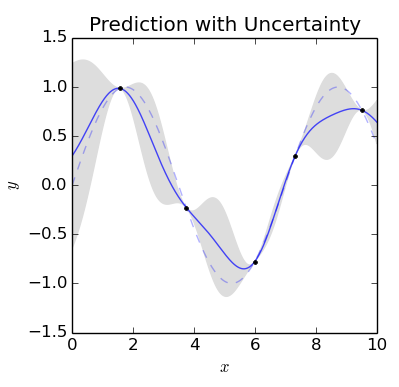
\includegraphics[width=0.4\linewidth]{Gaussian_Process_Regression.png}
	\caption{An illustration of a one-dimensional GP. The
		function used to generate the data points 
		is shown with the dashed line. The available data points are shown in
		black. The mean interpolated prediction is shown in blue
		along with the gray region showing the 68\% 
		credible interval. This figure is taken from Cdipaolo96 at 
		the Wikimedia Commons under the Creative Commons license 4.0
\label{fig:one_d_gaussian_process}}
\end{figure}
This shows the probabilistic nature of the GP predictions
(See Fig. \ref{fig:one_d_gaussian_process}).
Each drawn function represents one realization of the smoothed
field, which can be used to model the lensing observables derived 
from the lensing potential $\psi$ later on. 
By drawing many realizations of $\psi$, we can obtain the
corresponding credible levels.
Note that the credible levels are wider for regions with less data to reflect
the higher uncertainty. A GP is said to have indefinite dimension due to its ability to
predict values in unobserved regions, even though the 
observed part of the kernel is of finite size (e.g. $\ngal \times \ngal$). 
By averaging the drawn realizations, we can also obtain the mean prediction. 

[TODO fix this awkward paragraph] 
Compared with the past representation of
cosmic shear with summary statistics, the GP gives probabilistic realizations.  
The two-point correlation functions (2PCF), 
the power spectrum, the peak statistics, aperture mass statistic and others, 
which are more comparable to the parameters of the GP, such as the kernel, or the
mean predictions, than the GP itself. After drawing a particular realization of
the lensing observables from the GP, all the physical relationships still
applies. 


% The probabilistic nature of the GP highlights the main differences of our
% approach vs past analysis approaches. While past analysis computes summary 
% statistics, such as the correlation-function to represent the  

\subsection{Adapting the exponential squared kernel with lensing physics}
When the input data is mean-subtracted, we can use a zero mean function in the
GP and the covariance kernel completely specifies the GP. 
There are several families of commonly used covariance kernel.
The ones that are of the highest interest to cosmic shear modeling 
are stationary kernels that can capture 
the homogeneity and the isotropy of the data. This allows predicted spatial fields
$\psi$ to have consistent properties as the large-scale matter distribution.
%
One of such choices is the exponential squared kernel: 
\begin{equation}
	\kerngp(r^2) = \lambda^{-1} \exp\left(\frac{-r^2}{2 l^2}\right),
	\label{eq:exp_sq_kernel}
\end{equation}
where 
\begin{equation}
	r^2 \equiv (\xv - \yv)^T \Matrix{D} (\xv - \yv), 
\end{equation}
This kernel only depends on the
squared magnitude of distances between pairs of galaxy locations. 
This chosen form is therefore invariant
under translational and rotational transformations.
The metric $\Matrix{D}$ is taken to be a diagonal matrix in this discussion but  
can be generalized to account for anamorphic distortions. There are two
additional parameters that specifies the GP which we call $\gpparams =
[\lambda, l^2]$.
The precision parameter $\lambda$ affects the 
amplitude of the density perturbation, while the correlation length (or
the characteristic length scale) $l^2$ 
determines how fast the correlations between different spatial locations of the
field $\psi$ fall off as a function of the spatial distance. The parameter
$l^2$ therefore determines how smooth the spatial field $\psi$ is. When one
examines the marginal likelihood of a GP when fitting it to the data, 
one can see that there is a penalization term for preventing $l^2$ from
over smoothing or under smoothing the data.

Additionally, the exponential squared kernel is infinitely differentiable. This
differentiable kernel choice allows us to derive an analytical expression to
relate the different lensing observables to enforce a consistent representation.  
With the use of Born approximation in the linear regime, the scalar lensing potential $\psi$ is related to 
each of the lensing observables mentioned in chapter 1, e.g. 
$\lensparams \equiv [\kappa, \gamma_1, \gamma_2]$, via the following derivatives:
\begin{align}
\kappa &= \frac{1}{2}\left(\frac{\partial^2 \psi}{\partial x_1^2} +
\frac{\partial^2 \psi}{\partial x_2^2 }\right) 
= \frac{1}{2} (\psi_{,11} + \psi_{,22}),\\ 
\gamma_1 
&=\frac{1}{2}\left(\frac{\partial^2 \psi}{\partial x_1^2} - 
\frac{\partial^2 \psi}{\partial x_2^2}\right) 
= \frac{1}{2} (\psi_{,11} - \psi_{,22}), \\
\gamma_2 
&=\frac{1}{2}\left(\frac{\partial^2 \psi}{\partial x_1 \partial
x_2} + \frac{\partial^2 \psi}{\partial x_2 \partial x_1}\right)
= \frac{1}{2} (\psi_{,12} + \psi_{,21}), 
\end{align}
where we have defined the shorthand for spatial derivatives with
subscripts for $h,i,j,k = 1, 2$ after a comma.
Since the covariance operator is linear, we can interchange the order of
operation between the covariance operator and the differentiation operators. 
The resulting 4th derivatives of the covariance
kernels $\kerngp_{\rm GP}$ have the following forms: 
\begin{align}
	\label{eq:kernel_derivatives1}
	\Cov (\kappa(\xv), \kappa(\yv))
&= \frac{1}{4}\left(
\kerngp_{,1111} + \kerngp_{,1122} + \kerngp_{,2211} + \kerngp_{,2222}
\right), \\
\Cov(\kappa(\xv), \gamma_1(\yv)) &= \frac{1}{4}\left(
\kerngp_{,1111} + \kerngp_{,2211} - \kerngp_{,1122} - \kerngp_{,2222}
\right), \\
\Cov(\kappa(\xv), \gamma_2(\yv)) &= \frac{1}{4}\left(
\kerngp_{,1112} + \kerngp_{,2212} + \kerngp_{,1121} + \kerngp_{,2221}
\right),\\
\Cov(\gamma_1(\xv), \gamma_1(\yv)) &= \frac{1}{4}\left(
\kerngp_{,1111} - \kerngp_{,1122} - \kerngp_{,2211} + \kerngp_{,2222}
\right), \\
\Cov(\gamma_1(\xv), \gamma_2(\yv)) &= \frac{1}{4}\left(
\kerngp_{,1112} + \kerngp_{,1121} - \kerngp_{,2212} - \kerngp_{,2221}
\right), \\
\Cov(\gamma_2(\xv), \gamma_2(\yv)) &= \frac{1}{4}\left(
\kerngp_{,1212} + \kerngp_{,1221} + \kerngp_{,2112} + \kerngp_{,2121}
\right),
	\label{eq:kernel_derivatives2}
\end{align}
where
\begin{equation}
	\kerngp_{,hijk} = \frac{\partial^4 \kerngp}{\partial x_h \partial x_i
	\partial y_j \partial y_k}.
\end{equation}

With the definition of ${\bf X}_i$ as follows:
\begin{equation}
	\frac{\partial r^2}{\partial \xv_i} = -\frac{\partial
	r^2}{\partial \yv_i} =
	2 \Matrix{D}(\xv - \yv)_i \equiv 2{\bf X}_i,
\end{equation}
we can show that each entry $\nu_{,hijk}$ of $\kerngp_{,hijk}$ is
related to each entry $\nu$ of the original exponential squared kernel
$\kerngp$ by:
\begin{equation}
\nu_{,x_h x_i y_j y_k} = (\beta^4 X_h X_i X_j X_k -
\beta^3 (X_h X_i \Matrix{D}_{jk} \delta_{jk} + 5~{\rm perm.}) + \beta^2
(\Matrix{D}_{hj} \Matrix{D}_{ik}\delta_{hj}\delta_{ik} + 2~{\rm perm.})) \nu,
\label{eq:4thderivatives}
\end{equation}
with $\beta = l^{-2}$. There are 6 permutations (abbreviated as perm.) of the terms in
eq. \ref{eq:4thderivatives}
multiplied to $\beta^3$ as we can choose two pairs of indices from the $h,i,j,k$ 
when we differentiate the terms by parts, assuming that the order of each
pair of indices matters. 
Likewise, there are 3 possible permutations of
the terms the multiplied to $\beta^2$ as we can choose two pairs of indices from
$h, i, j, k$ where the order of the pairs does not matter.
The derivation of the relevant derivatives and terms are available 
in appendix \ref{app:GP_kernel_derivation} for completeness. 
Our implementation of the GP kernels in eqn \ref{eq:kernel_derivatives1} - 
\ref{eq:kernel_derivatives2} is also openly available at
\href{https://github.com/karenyyng/george}{https://github.com/karenyyng/george}.

\subsection{Making predictions (interpolation) with a GP}

\begin{figure}
	\centering
	\includegraphics[width=0.8\linewidth]{gp_cov_v2.png}
	\caption{An illustration of the GP covariance kernel for the data set
		presented in Schneider et al. (in prep.). We can see the various covariance
		and cross-covariance
		structures for the training data $\Upsilon = [\kappa, \gamma_1, \gamma_2]$
		and the interpolated data $\Upsilon' = [\kappa', \gamma_1', \gamma_2']$.
		\label{fig:GP_kernel_vis}}
\end{figure}
Using a GP instead of a summary statistic also allows us to make predictions. 
We know the joint probability density function for the observables of a GP to
be:
\begin{equation}
	[\lensparams',\lensparams]^T \sim \mathcal{N}(0, \kerngp_{\rm GP})
\end{equation}
where $(\lensparams', \xv')$ represents the unobserved set of data,
and the $(\lensparams, \xv)$ represents the existing (training) data.
We can then represent the kernel matrix in terms of several submatrices 
(See Fig. \ref{fig:GP_kernel_vis} for an example):
\begin{equation}
	\kerngp_{\rm GP} = \left[\begin{array}{cc}
	A & B \\
	B^T & C 
\end{array} \right].	
\end{equation}
We can prove that the different observations from a multivariate Gaussian are 
conditionally independent with the use of the Schur complement to give the following:
\begin{equation}
	\mathbb{E}(\lensparams'|\lensparams) = \mathbb{E}(\lensparams) + BC^{-1}(\lensparams - \mathbb{E}(\lensparams))
\end{equation}
and
\begin{equation}
	\Cov(\lensparams'|\lensparams) = A - BC^{-1}B^T
\end{equation}
which enables us to draw new predictions $\lensparams'$ from the conditional distribution:
\begin{equation} 
	\lensparams' | \xv', \xv, \lensparams \sim \mathcal{N}(
		\mathbb{E}(\lensparams'| \lensparams), \Cov(\lensparams'|\lensparams)
	)
\end{equation}
In the presence of shape noise and measurement uncertainties, the actual 
expression of the conditional covariance kernel used for interpolation in the actual analysis 
is slightly more complicated as we will show. 
But the general idea of the above derivation follows 
since we also assume the shape noise and the measurement uncertainties to be Gaussian.

Similarly, once we can find GP parameters $\gpparams^*$ that optimizes the fit to
the observed shear fields $\gamma_{(1, 2)}$ at $\xv$, we can compute $\kerngp_{(\kappa,
\kappa)}$ and draw predictions of $\kappa$ from the conditional distribution. 
Compared with an interpolation method, the mean predictions from a GP are
often more well behaved and do not show drastic increase or decrease 
in the tail regions where there is no data.  

\subsection{Performing cosmic shear inference with a GP}
\begin{figure}
	\centering
	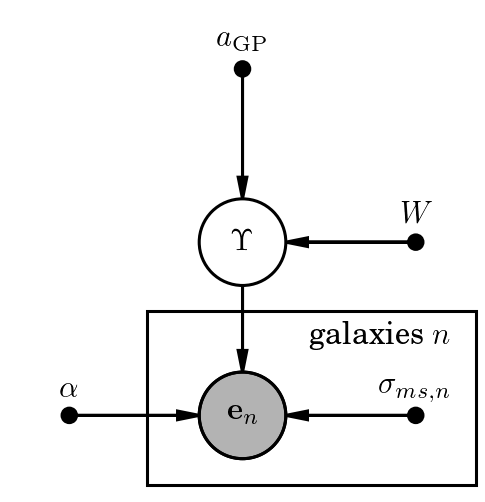
\includegraphics[width=0.4\linewidth]{shear_gp_pgm.png}
	\caption{A simplified probabilistic graphical model (pgm) for inferring
		the lensing observables $\Upsilon$ from survey or simulation data. The dots
		denote fixed parameters in the statistical procedure. The circle denotes
		latent variable, while the shaded circle denotes 
		the observed variable. The plate notation shows the galaxy entries to sum
		over.
		\label{fig:simplified_pgm}}
\end{figure}

\begin{figure}
	\centering
	\includegraphics[width=0.4\linewidth]{shear_general_pgm.png}
	\caption{A more general probabilistic graphical model (pgm) for inferring
		the lensing observables $\Upsilon$. The circle denotes
		latent variable, while the shaded circle denotes 
		the observed variable. The plate notation shows the galaxy entries to sum
		over.
		\label{fig:general_pgm}}
\end{figure}


\subsubsection{Specifying the GP prior}
Throughout the analyses present in this work, 
we make use of the weak shear approximation 
$g = \gamma / (1 - \kappa)  \approx \gamma$, so the observed ellipticity can be
written as: 
\begin{equation}
	\epsilon_{\rm obs} = \epsilon_{\rm int} + g 
\end{equation}
Assume that the shape noise term $\epsilon_{\rm int}$ of each galaxy is 
independent and follow the same Gaussian distribution, we can model  
the shape noise ($\sigma_e$) and measurement uncertainty ($\sigma_{\rm ms}$)
as part of a composite GP kernel. 
\begin{equation}
	\mathsf{S} = \kerngp_{GP} + \sigma_e^2 \mathds{1} + \sigma_{\rm ms}^2
	\mathds{1}   
\end{equation}


\subsubsection{Formulating the likelihood}

\subsection{Validation data}
\subsubsection{{\sc GalSim} data}

\subsubsection{Data centered on the Deep Lens Survey (DLS) galaxy cluster Abell 781}
We illustrate that the GP can handle non-linear structures such as a galaxy cluster 
by making a mass map of Abell 781 in the DLS. 



\section{Results}
 \begin{figure}
	\centering
	\includegraphics[width=0.7\linewidth]{mass_map_comparison_galsim.png}
	\caption{A comparison of mass maps for simulated inputs from {\sc GalSim} and
	the mass map generated with the use of a GP prior \label{fig:Galsim_massmaps}. 
	This figure is part of Schneider et al. (in prep.).
}
\end{figure}

\begin{figure}
	\centering
	\includegraphics[width=0.4\linewidth]{kappa_Abell781.png}
	\includegraphics[width=0.4\linewidth]{kappa_Abell781_WD.png}
	\caption{A comparison of mass maps for Abell 781 in the Deep Lens Survey (DLS) 
		\label{fig:Abell781_massmap}.  Left: The smoothed mass map of Abell 781 from 
		Right: The output generated with 6000
		galaxies. 
	These figures are part of Schneider et al. (in prep.).
}
\end{figure}



\begin{table}%[htb]
% \small
\begin{center}
\caption{Parameters for the statistical model.}
\label{tab:sampling_parameters}
\begin{tabular}{cl}
\hline
Parameter & Description \\
\hline
${\bf d_{n}}$ & data vector (measured $e_{1,2}$ for each galaxy $n$)  \\
$\sigma_{{\rm ms}; n}$ & ellipticity measurement error for galaxy $n$ 
\\
$\xv$, $\yv$ & vector(s) of 2D spatial locations of galaxies \\
$\epsilon_n^{\rm int}$ & intrinsic galaxy ellipticity for galaxy $n$ \\
$\alpha\equiv\sigma_{e}^2$ & parameters of the distribution of galaxy parameters \\
W & window function for the survey footprint \\
$\lensparams$ & lensing shear and convergence ($\gamma_{1,2}, \kappa$) \\
$\gpparams$ & parameters of the GP kernel\\
% $\rho_{\rm GP}$ & correlation of the GP kernel (element of $\gpparams$) \\
$\lambda$ & precision of the GP kernel (element of $\gpparams$) \\
$l^2$ & squared GP correlation length (element of $\gpparams$) \\
% $\lambda_{\epsilon}$ & precision for the nugget term (element of $\gpparams$) \\
\hline
\end{tabular}
\end{center}
\end{table}



\subsection{Verification using {\sc GalSim} simulated data}
\subsection{Mass mapping for Deep Lens Survey Abell 781}

% Is a non-trivial optimization problem 

\section{Discussion}

\subsection{Comparison of our method to other approaches}
  Since our project wants to specify 
% The main difficulty of this project, 

The joint PDF can carry more information,
such as the uncertainties from the inputs, 
than summary statistics. 
A mature current approach to summarize the matter distribution 
involves computing a statistic, such
as the two-point correlation function (2PCF) for each of the lensing
observables, including the convergence and the two components of shear, 
$\Upsilon = [\kappa, \gamma_1, \gamma_2]$. 
An implementation of the 2PCF from \cite{Jee2013a} is: 
\begin{equation}
	\xi_\Upsilon(\theta) = \frac{\sum_{i,j}w_i, w_j e_i, e_j}{\sum w_i, w_j}.
	\label{eqn:2PCF}
\end{equation}
This expression is computed 
for all pairs of source galaxies with subscripts $i < j$ at an angular separation 
$\theta$, and $w_{(i, j)}$ is usually
a weight factor taken to be a function of 
the inverse of the measurement uncertainty $\sigma_{ms; (i, j)}$.  
A closely related quantity is the Fourier transform of the 2PCF, which consists
of the power spectrum. For a Gaussian random field, the power spectrum contains
all the information about the Gaussian random field. 

Other statistic that have been explored for capturing cosmic shear information
include aperture mass dispersion $M_{\rm ap}$ or shear peak count \citep{Bard2014}.


\subsection{The computational performance of our method}
We implemented the covariance kernels in \ref{eq:kernel_derivatives1}
via {\sc C++} along with a {\sc Python} wrapper. 
Although the operation of computing and assembling the
derivatives are $O(\ngal^2)$, the large number of addition and 
multiplication operations can be slow in eq. [TODO].
Exploiting the symmetry of the covariance kernel can only provide 
memory saving of a factor of 2.
To make the computation feasible, 
I implemented the parallelized computation of each element of the kernel using 
the {\sc OpenMP} library. The slowest step of the entire computation, however, 
is the inversion of the
covariance kernel matrix for the evaluation of the marginal likelihood in eqn.
[TODO], 
which is an $O(\ngal^3)$ operation. 
I made use of a parallelized version of the Cholesky decomposition via the {\sc Intel Math
Kernel Library} to invert the matrix and achieved $\sim10$ 
times speed up so the
computation and the evaluation of the likelihood of each set of GP parameter
take $< 10s$ for 1600 galaxies, which translates to 
the inversion of a 4200 $\times$ 4200 covariance matrix.
With the use of distributed computational resources, it is possible 
to probe the space of possible GP parameters.  

Currently, our method is not as computationally competitive as the 2PCF. One of
the fastest implementation of 2PCF has a computational complexity of $O(N\sqrt{N})$.
The 2PCF algorithm has also been demonstrated to scale almost linearly with
computational resources 
with a distributed and parallelized implementation \citep{Chhugani2012}.

Rather than relying on manual intensive methods for parallelizing the
computation of the kernel methods, a more promising way is to approximate the
small elements in the covariance kernel structure as zero. 

The relevant field of literature about how approximating the kernel as a sparse
matrix may affect the
statistical inference is called covariance tapering. 
On the other hand, \citep{Snelson2006}
there are papers demonstrating that synthetic data with much less data points  
would produce further 
With large amount of
sparsity, the inversion of the matrix can be sped up to [TODO]$O(M^2N)$ for
building the model and $O(M^2)$ for interpolating / predicting output functions
at new input locations \citep{Snelson2006}.
  



\subsection{Alternative kernel choice(s) for encoding the lensing physics}
Alternative choices for a covariance kernel for describing the lensing physics 
include the family of Mat\'{e}rn kernels:
\begin{equation}
	\kerngp(\xv, \xv') = \frac{1}{\Gamma(\nu)2^{\nu-1}}\left[
		\frac{\sqrt{2\nu}}{l}|\xv - \xv'|
	\right]^\nu K_\nu \left(\frac{\sqrt{2\nu}}{l}|\xv-\xv'|\right) 
\end{equation}
where $K_\nu$ is the modified Bessel function of the second kind, with an order
$\nu$, whereas $l$ is the characteristic length scale.
The smoothness of the data generated from a Mat\'{e}rn kernel is closely
related to the degree of freedom $\nu$ of the kernel. 
The higher degree of freedom it has, the smoother the spatial variations of the
drawn $\psi$ would be for the same characteristic length scale $l$.
Note that a Mat\'{e}rn kernel is also only differentiable to the $(\nu-1/2)$ order.
This restricts us to use kernels with $\nu > 9/2$ . 
When we take the limit of the degree of freedom of a Mat\'{e}rn kernel to infinity, 
we recover the exponential squared kernel. The inclusion of a Mat\'{e}rn kernel
in addition to an exponential squared kernel, therefore, will pick up features
that are less smooth.

As the manual differentiation of the analytical form of the kernels can be tedious,
it may desirable to generalize the derivation of derivatives. Technologies such
as automatic differentiation 
can spreads factors of the derivatives over a tree structure for
almost exact computation.
 
% An implementation via numerical differentiation may
% or may not be more computationally intensive to
% compute, depending on the required numerical precision (aka order of accuracy).




% \subsection{Relating the lensing observables to a cosmological model}
% We can draw realizations of the lensing observables from the GP given a set of
% optimized GP parameters:
% \begin{equation}
% 	\lensparams(\xv) \sim GP(0, \kerngp_{\rm GP}(\xv, \yv)) 
% \end{equation}
% 
% 
% The constraints on cosmological parameters need to be verified in a mock
% weak-lensing analysis of cosmological simulation. 
% It can enable the separation of E and B mode in the convergence field as shown
% in Schneider et al. (in prep.) 

\subsection{Modeling the systematics and noise via a composite kernel}
Besides kernels that describes homogeneous and isotropic data,
there are other types of periodic kernels that may be useful
in modeling systematics such as masking or footprints of the telescope due to the
stacking of multiple exposures.
For spatial models with undetermined periodicity or patterns, 
composite kernels with different covariance structures 
can be formed by the addition and/or multiplication of several kernels,
\begin{equation}
	\kerngp = \sum_i \kerngp_i(\gpparams^i).
\end{equation}
By fitting for the best values for $\gpparams^i$, it is possible  
to pick up (sometimes non-obvious) patterns in the data \citep{Duvenaud2013},
and in this case, the two shear components. 

% - [ ] describe why the lensing observables shouldn't have a B mode 
% Since the lensing observables are the second derivatives of a scalar field,
% it is known that they should be curl free and only contain E-mode signal. 

% It is well known that gravitational lensing, as presented in chapter 1,
% only induces a curl-free (E-mode) shear signal. However, the computation of 
% summary statistics at certain length scale can induce a B-mode (with non-zero
% curl) signal. 

%  \begin{align}
% 	\kappa^E & = \kappa\\
% 	\kappa^B & = 0 \\
% 	\gamma^E &= \left[\frac{1}{2} (\psi^E_{,11} - \psi^E_{,22}) -
% 	\psi^B_{,12}\right]\\
% 	\gamma^B &= \left[\psi^E_{,12} + \frac{1}{2} (\psi^B_{,11} - \psi^B_{,22})\right]
% \end{align}
% Can handle sharp boundaries from stacking images 
% cite Jee2013a  
% cite Rowe2010 paper for interpolating star fields for 
% PSF ellipticity corrections 

\section{Conclusion}
Here, we have derived and implemented a fully probabilistic method for 
representing the lensing observables.   

The potential of using a Gaussian Process for the inference of cosmological 
Gaussian Process (GP)parameters remains to be proved. 
Some of the remaining challenges include the generalization of the method for spherical
coordinates. 


Requires the understanding of the underlying physical observable, how the statistical
approach can carry the information and how to actual execute the computation in
a tractable way.


\section{Acknowledgement}
We thank Chris Paciorek for discussion about the statistical
framework for performing shear inference and the
use of Gaussian Processes.
This research
used the resources of the National Energy Research Scientific 
Computing Center (NERSC), a DOE Office of Science
User Facility supported by 
of the U.S. Department of Energy under Contract No.
DE-AC02-05CH11231.
 This work uses a modified version
of the public code {\sc George} available at \href{https://
github.com/karenyyng/george}{https://
github.com/karenyyng/george}, which was forked from \\
\href{https://github.com/dfm/george}{https://github.com/dfm/george}.



\appendix 

\section{Derivation of GP kernel}
\label{app:GP_kernel_derivation}


\subsection{The relevant 4th spatial derivatives}
We show how to derive one of the 6  covariance matrices that we can compute
from $\lensparams = [\kappa, \gamma_1, \gamma_2]$. The computation of the other
covariance kernels is completely analogous.
\begin{align*}
&{\rm Cov}_{m,n} (\kappa(\vec{x}), \kappa(\vec{y}))  \\ 
&= \mathbb{E} \left[ 
	(\kappa - \mathbb{E}[\kappa])|_m 
( \kappa - \mathbb{E}[\kappa])|_n\right] 
\\
 &=\mathbb{E}\left[
\frac{1}{2} \left(\frac{\partial^2}{\partial y_1^2} + 
\frac{\partial^2}{\partial y_2^2}\right) 
 (\psi - \mathbb{E}\left[\psi\right])|_n \frac{1}{2}
\left(\frac{\partial^2}{\partial x_1^2} + \frac{\partial^2}{\partial x_2^2} \right)
(\psi - \mathbb{E}\left[\psi\right])|_m \right]
\\
&= \frac{1}{4}\left(
\frac{\partial^2}{\partial x_1^2} \frac{\partial^2}{\partial y_1^2} + 
\frac{\partial^2}{\partial x_1^2} \frac{\partial^2}{\partial y_2^2} +  
\frac{\partial^2}{\partial x_2^2} \frac{\partial^2}{\partial y_1^2} + 
\frac{\partial^2}{\partial x_2^2} \frac{\partial^2}{\partial y_2^2}  
\right) \kerngp_{mn}\\ 
\end{align*}


\subsection{The actual terms from the 4th derivatives}
\begin{equation*}
\kerngp = \lambda^{-1} \Sigma 
\end{equation*}

\begin{align}
\Sigma &= \exp{\left(\frac{-\beta}{2} r^2 \right)}\\
\Sigma_{,x_i} &= \frac{-\beta}{2} \Sigma r^2_{,x_i} = -\beta \Sigma X_i\\ 
\Sigma_{,y_h} &= \beta \Sigma X_h 
\end{align}

\begin{align}
\Sigma_{,x_i x_j} &= \frac{-\beta}{2}(\Sigma_{,x_j} r^2_{,x_i} + \Sigma r^2_{,x_i x_j})\\
\Sigma_{,x_i x_j y_h} &= \frac{-\beta}{2}(\Sigma_{,x_j y_h} r^2_{,x_i} + \Sigma_{,x_j}
r^2_{,x_i y_h} + \Sigma_{,y_h} r^2_{,x_i x_j})\\
\Sigma_{,x_i x_j y_h y_k} &= \frac{-\beta}{2} 
(\Sigma_{,x_j y_h y_k} r^2_{,x_i} +
\Sigma_{,x_j y_h} r^2_{,x_i y_k} + 
\Sigma_{,x_j y_k} r^2_{,x_i y_h} + 
\Sigma_{,y_h y_k} r^2_{,x_i x_j} )
\label{eq:4th_derivative_intermediate_expression}
\end{align}

Just work on terms that are parts of the 4th kernel derivative 
\begin{align*}
\Sigma_{,x_i x_j} &= \frac{\partial}{\partial x_j} (-\beta \Sigma X_i)\\
&= -\beta(\Sigma_{,x_j X_i} + \Sigma X_{i, x_j})\\ 
&= -\beta(-\beta \Sigma X_j X_i + \Sigma \delta_{ij} \mathsf{D}_{ij}) \\ 
&= (\beta^2 X_j X_i - \beta \delta_{ij} \mathsf{D}_{ij})\Sigma 
\end{align*}

\begin{align*}
\Sigma_{,x_i y_h} &= \frac{\partial}{\partial y_h} (-\beta \Sigma X_i)\\
&= -\beta(\Sigma_{,y_h X_i} + \Sigma X_{i, y_h})\\ 
&= -\beta(\beta \Sigma X_h X_i - \Sigma \delta_{ih} \mathsf{D}_{ih}) \\ 
&= -(\beta^2 X_h X_i - \beta \delta_{ih} \mathsf{D}_{ih})\Sigma 
\end{align*}

\begin{align*}
\Sigma_{,y_h y_k} &= \frac{\partial}{\partial y_h} (\beta \Sigma X_h)\\
&= \beta(\Sigma_{,y_k X_h} + \Sigma X_{h, y_k})\\ 
&= \beta(\beta \Sigma X_k X_h - \Sigma \delta_{hk} \mathsf{D}_{hk}) \\ 
&= (\beta^2 X_h X_k - \beta \delta_{hk} \mathsf{D}_{hk})\Sigma 
\end{align*}

\begin{align}
\Sigma_{,x_i x_j} &= (\beta^2 X_j X_i - \beta \delta_{ij} \mathsf{D}_{ij})\Sigma\\ 
\Sigma_{,x_i y_h} &= -(\beta^2 X_h X_i - \beta \delta_{ih} \mathsf{D}_{ih})\Sigma\\ 
\Sigma_{,y_h y_k} &= (\beta^2 X_h X_k - \beta \delta_{hk} \mathsf{D}_{hk})\Sigma 
\end{align}

Term 1 of the 4th derivative of eqn \ref{eq:4th_derivative_intermediate_expression}

\begin{align*}
\Sigma_{,x_j y_h y_k}
&= \frac{\partial}{\partial y_k} \Sigma_{,x_j y_h}\\ 
&= -\frac{\partial}{\partial y_k} (\beta^2 X_h X_j - \beta \delta_{jh} \mathsf{D}_{jh})\Sigma\\
&= (\beta^2 \mathsf{D}_{hk} \delta_{hk} X_j + \beta^2 X_h \mathsf{D}_{jk}\delta_{jk})\Sigma -
(\beta^2 X_h X_j - \beta \mathsf{D}_{jh} \delta_{jh})\beta X_k \Sigma
\end{align*}

\begin{align*}
&\Sigma_{,x_j y_h y_k} r_{,x_i}^2\\
&= 2[\beta^2 X_j \mathsf{D}_{hk} \delta_{hk} + \beta^2 X_h \mathsf{D}_{jk}\delta_{jk} +
\beta^2 X_k \mathsf{D}_{jh} \delta_{jh} - \beta^3 X_h X_j X_k] X_i \Sigma\\ 
&=\boxed{2\beta^2[ 
X_j X_i \mathsf{D}_{hk} \delta_{hk} + 
X_h X_i \mathsf{D}_{jk} \delta_{jk} + 
X_k X_i \mathsf{D}_{jh} \delta_{jh}] \Sigma 
- 2\beta^3 X_h X_j X_k X_i \Sigma} 
\end{align*}

\subsection{Term 2 of the 4th derivative}
\begin{align*}
\Sigma_{,x_j y_h} r^2_{,x_i y_k}
&= - (\beta^2 X_h X_j - \beta \mathsf{D}_{jh} \delta_{jh}) (-2\mathsf{D}_{ik}
\delta_{ik} \Sigma) \\  
&= \boxed{( 2 \beta^2  X_h X_j \mathsf{D}_{ik} \delta_{ik} 
-2 \beta \mathsf{D}_{jh} \mathsf{D}_{ik} \delta_{jh} \delta_{ik}) \Sigma} 
\end{align*}

\subsection{Term 3 of the 4th derivative}
This is completely analogous to term 2 except the subscripts are slightly
different
\begin{align*}
\Sigma_{,x_j y_k} r^2_{,x_i y_h}
&=\boxed { ( 2 \beta^2  X_k X_j \mathsf{D}_{ih} \delta_{ih} 
-2 \beta \mathsf{D}_{jk} \mathsf{D}_{ih} \delta_{jk} \delta_{ih}) \Sigma} 
\end{align*}

\subsection{Term 4 of the 4th derivative} 
\begin{align*}
\Sigma_{,y_h y_k} r^2_{,x_i x_j}
&= (\beta^2 X_k X_h - \beta \mathsf{D}_{hk}\delta_{hk})\Sigma 2 \mathsf{D}_{ij} \delta_{ij}\\ 
&= \boxed{(2\beta^2 X_k X_h \mathsf{D}_{ij} \delta_{ij} - 2\beta \mathsf{D}_{ij} \mathsf{D}_{hk} \delta_{hk}
\delta_{ij})\Sigma } 
\end{align*}

Collecting terms of $\Sigma_{,x_i x_j y_h y_k}$ by plugging them in eqn
\ref{eq:4th_derivative_intermediate_expression}
, we have 
\begin{align}
\nu_{,x_i x_j y_h y_k} &= (\beta^4 X_h X_j X_k X_i -  
\beta^3 (X_j X_i \mathsf{D}_{hk} \delta_{hk} + 5 {\rm perm.}) + \beta^2
(\mathsf{D}_{jh} \mathsf{D}_{ik}\delta_{jh}\delta_{ik} + 2 {\rm perm.})) \nu \\
&= \gamma \nu
\end{align}
where $\nu$ is an entry in the matrix $\Sigma$.

